\hypertarget{03-visual-computing-i-ch018}{}
\chapter{18 --- C++ Representation, Ownership and Lifetime}\label{03-visual-computing-i-ch018-c-representation-ownership-and-lifetime}

\hyperref[volume-reading-map]{Reading map} · \hyperref[03-visual-computing-i-ch017]{Previous chapter} · \hyperref[03-visual-computing-i-ch019]{Next chapter}

C++ correctness relies on representation invariants, ownership and object lifetime, not syntax alone. These sections use assignments and no-throw properties to reason about resource-safe changes.

\textbf{By the end:} Use representation and lifetime invariants to assess C++ resource operations.

\textbf{Recall question:} Why can a no-throw move change the safety of container growth?

\section{Reconstruct the representation and lifetime proofs}\label{03-visual-computing-i-ch018-reconstruct-the-representation-and-lifetime-proofs}

\section{C++ - Assignment as a resource transaction}\label{03-visual-computing-i-ch018-c---assignment-as-a-resource-transaction}

The \href{../01-Foundations-I/main.pdf\#nameddest=appendix-bea6beb5350f}{strong guarantee (01-Foundations-I, appendix-bea6beb5350f)} requires a defined observable state before the operation and an unchanged promised state if preparation fails. Let D0 be the destination's original owned allocation/value and S the source. The teaching byte owner's copy assignment follows:

\begin{enumerate}
\def\labelenumi{\arabic{enumi}.}
\tightlist
\item
  Construct replacement R from S without changing D0. Allocation failure propagates while D0 and S retain their original state.
\item
  Non-throwing swap transfers R's value into the destination and D0 into the temporary. This is the commit point: no remaining step can fail under the stated byte-copy/release contract.
\item
  Destroy R, releasing the former destination D0 exactly once.
\end{enumerate}

Self-copy is explicitly guarded; an alternative copy-and-swap without that guard could still be safe but allocate unnecessarily. This proof assumes a non-throwing swap, safe release, and copy preparation that does not mutate its source. It does not establish whole-object strong guarantees for arbitrary memberwise assignment or a copy operation with external side effects.

For the failure-injection witness, initial owners A/B each hold one allocation. An injected exception before the new allocation succeeds leaves two owners/two live allocations and B's old byte9. Moving A into C then leaves A empty while C owns A's allocation. Moving C into B releases B's previous allocation before adoption, leaving one allocation. Destroying/resetting its final owner leaves zero. The source remains a live empty object throughout its moved-from interval.

\subsection{Why no-throw properties matter to growth}\label{03-visual-computing-i-ch018-why-no-throw-properties-matter-to-growth}

Suppose source element0 is moved and changed, then moving element1 throws. The partially populated new buffer can be cleaned up, but cleanup alone does not restore element0's old value. Copying that preserves source state can support rollback where available; a genuinely non-throwing move avoids that transfer failure. If copying is unavailable and moving may throw, consult the exact operation's exceptional-effects contract. move\_if\_noexcept encodes the relevant construction-expression choice, not a universal rollback theorem.

\subsection{Isolating sink counts from growth}\label{03-visual-computing-i-ch018-isolating-sink-counts-from-growth}

With spare destination capacity and a Probe type whose copy/move constructors are instrumented: lvalue→value parameter→element gives one copy/one move; xvalue→parameter→element gives two moves; same-type prvalue→parameter→element gives direct parameter construction/one move. Cache growth would add transfer of old elements. Optional named-result NRVO is independent of these parameter routes, so record it separately instead of silently adding it to a fixed portable count.

\section{C++ - Qualification safety and borrow intervals}\label{03-visual-computing-i-ch018-c---qualification-safety-and-borrow-intervals}

\subsection{Why nested const needs an intermediate guard}\label{03-visual-computing-i-ch018-why-nested-const-needs-an-intermediate-guard}

This is a hypothetical proof by contradiction, not legal code to run. Suppose \texttt{int**} could convert to \texttt{const\ int**}:

\begin{verbatim}
const int immutable = 7;
int* mutable_path = nullptr;
int** outer = &mutable_path;
// const int** injected = outer; // actual C++ rejects this
// *injected = &immutable;       // hypothetical mutation of mutable_path
// *mutable_path = 9;            // would write an actually const object
\end{verbatim}

Step one establishes a const object. Step two gives the mutable pointer a mutable type. The hypothetical conversion lets a const-object address enter that mutable pointer through an alias. The final write would violate the first promise without an explicit cast. Therefore adding const only at the deepest level is not safe. \texttt{const\ int*\ const*} makes the intermediate pointer read-only through that path, rejecting the injection assignment. This explains the safety requirement; the general language rule is qualification decomposition, not a special ban against double pointers. See \href{../01-Foundations-I/main.pdf\#nameddest=appendix-5e1a7561cd98}{Multilevel pointer qualification (01-Foundations-I, appendix-5e1a7561cd98)}.

\subsection{A borrow's access interval is an intersection}\label{03-visual-computing-i-ch018-a-borrows-access-interval-is-an-intersection}

Let \(L_o\) denote times at which the referent is live, \(L_s\) times at which its storage/access relationship is valid, and \(L_i\) times at which the path still names the intended logical entity. Under the API's mutation and synchronization contract, the admissible access times satisfy:

\[
L_{\mathrm{access}}\subseteq L_o\cap L_s\cap L_i.
\]

These are sets of times, not byte counts or durations to add. Const/type/bounds/permissions still add independent obligations. Reallocation can end the old storage relationship; destruction ends the old object's live interval; slot assignment can preserve the live object while ending its association with a logical entity. A non-null bit pattern establishes none of those intervals.

For an epoch witness, save \(e_b\) when borrowing and compare with the live pool epoch \(e_p\) before access. Acceptance requires \(e_b=e_p\), but that test is meaningful only if the epoch owner remains live, every invalidating mutation advances the counter, equality cannot falsely recur through wrap, and mutation cannot race between check and use. A single-threaded epoch implements a conservative API contract, not a proof of ownership or lock-free safety. See \href{../01-Foundations-I/main.pdf\#nameddest=appendix-aa405b7c3903}{Borrow contracts and pool epochs (01-Foundations-I, appendix-aa405b7c3903)} and the inline \href{../01-Foundations-I/main.pdf\#nameddest=01-foundations-i-ch003-when-a-valid-borrow-stops-naming-the-intended-thing}{slot trace (01-Foundations-I, 01-foundations-i-ch003-when-a-valid-borrow-stops-naming-the-intended-thing)}.

\subsection{Forwarding reconstructed from collapsing}\label{03-visual-computing-i-ch018-forwarding-reconstructed-from-collapsing}

For an lvalue argument of type int to deduced \texttt{T\&\&}, deduction chooses \texttt{T=int\&}; applying \texttt{\&\&} to that substituted reference collapses to \texttt{int\&}. For an int prvalue, deduction chooses \texttt{T=int}; the parameter is \texttt{int\&\&}. In the body the parameter's name is an lvalue in both cases. \texttt{std::forward\textless{}T\textgreater{}} uses the deduced T to restore the original category; unconditional move discards that distinction. This derivation requires the forwarding pattern, not merely any spelling containing two ampersands.

\section{C++ - Conventional record layout and identity horizon}\label{03-visual-computing-i-ch018-c---conventional-record-layout-and-identity-horizon}

This proof extends \href{../01-Foundations-I/main.pdf\#nameddest=01-foundations-i-ch003-bringing-the-object-model-back-to-bytes}{the inline layout explanation (01-Foundations-I, 01-foundations-i-ch003-bringing-the-object-model-back-to-bytes)}, not a universal class-layout algorithm. Assume an ordinary ABI with member size/alignment pairs, no bases, virtual machinery, overlap, packing or stronger requested alignment. For nonnegative offset x and positive required alignment a:

\[
\operatorname{roundUp}(x,a)=a\left\lceil\frac{x}{a}\right\rceil.
\]

Place each member at its rounded-up offset, advance by its size, then round the complete extent to the ABI's class alignment. For char/double/char with sizes 1/8/1 and alignments 1/8/1: first offset0; double roundUp(1,8)=8; final char offset16; extent17; size roundUp(17,8)=24. Reordering double/char/char gives offsets0/8/9, extent10 and size16. Adjacent array elements then begin at aligned multiples of the complete size. This is a target model to measure, not the meaning of standard-layout.

A generation counter of G bits has 2\^{}G possible bit patterns. If one slot is reused r times per second, a wrap horizon under steady reuse is:

\[
T=\frac{2^G}{r}.
\]

T is in seconds when r is reuses/second. This predicts counter wrap, not guaranteed collision freedom: a retained old handle may match again after wrap, and a handle from another registry can match sooner. Reserve invalid states, width choice and reuse/quarantine policy can change the horizon. A validity check must include the owning registry and live slot state.

Neither proof makes a C++ object's physical address its semantic identity. Neither grants pointer arithmetic across adjacent non-array members.

Extended mathematical and logical derivations live here under durable concept headings. Update an existing derivation when a later chunk adds assumptions, a more general form, limiting cases, or corrections.

Each derivation records:

\begin{itemize}
\tightlist
\item
  the main-note chunk that first requires it;
\item
  definitions, domains, units, conventions, and assumptions;
\item
  every non-obvious step;
\item
  dimensional, sign, boundary, and limiting-case checks;
\item
  links to later chunks that deepen or reuse it.
\end{itemize}

\section{M001 - Positional value, masks, fields, and De Morgan}\label{03-visual-computing-i-ch018-m001---positional-value-masks-fields-and-de-morgan}

\textbf{Introduced by:} \href{../01-Foundations-I/main.pdf\#nameddest=01-foundations-i-ch001-from-a-signal-to-an-interpretation}{C001 / M001 (01-Foundations-I, 01-foundations-i-ch001-from-a-signal-to-an-interpretation)}

\subsection{Unsigned positional value and base conversion}\label{03-visual-computing-i-ch018-unsigned-positional-value-and-base-conversion}

For bits \(b_i\in\{0,1\}\), an unsigned \(N\)-bit pattern means

\[
V=\sum_{i=0}^{N-1}b_i2^i.
\]

Euclidean division gives \(n=2q+r\), with \(r\in\{0,1\}\). Therefore \(r=b_0\); repeating on \(q\) exposes \(b_1,b_2,\ldots\), so remainders arrive LSB-first. Decoding left-to-right uses the Horner recurrence \(v\leftarrow2v+b\).

Check for \texttt{10101101}: \(128+32+8+4+1=173\). Repeated division of 173 returns remainders \texttt{1,0,1,1,0,1,0,1}, whose reverse is \texttt{10101101}.

\subsection{Contiguous masks, extraction, and insertion}\label{03-visual-computing-i-ch018-contiguous-masks-extraction-and-insertion}

A width-\(w\) low mask is

\[
L_w=2^w-1
\]

because \(2^w\) is \texttt{1} followed by \(w\) zeros and subtracting one borrows through them to produce \(w\) ones. Moving the field to offset \(s\) gives \(M=L_w\ll s\).

Extraction first normalizes, then isolates:

\[
extract(x,s,w)=(x\gg s)\land L_w.
\]

Insertion must preserve every position outside \(M\). The term \(x\land\neg M\) clears exactly the destination; \((v\land L_w)\ll s\) encodes only values representable by the field. Since their 1-bits cannot overlap outside the destination,

\[
insert(x,v,s,w)=(x\land\neg M)\lor((v\land L_w)\ll s).
\]

Implementation checks: \(w>0\), \(s+w\le N\), shifts are smaller than the carrier width, and complement is evaluated at carrier width. A semantic API must choose whether an oversized \(v\) is rejected or truncated.

\subsection{De Morgan by exhaustive truth assignment}\label{03-visual-computing-i-ch018-de-morgan-by-exhaustive-truth-assignment}

For two Boolean inputs there are only four assignments. Evaluating both sides on \texttt{(0,0)}, \texttt{(0,1)}, \texttt{(1,0)}, and \texttt{(1,1)} yields identical result columns:

{\def\LTcaptype{none} % do not increment counter
\begin{longtable}[]{@{}
  >{\raggedleft\arraybackslash}p{(\linewidth - 10\tabcolsep) * \real{0.1667}}
  >{\raggedleft\arraybackslash}p{(\linewidth - 10\tabcolsep) * \real{0.1667}}
  >{\raggedleft\arraybackslash}p{(\linewidth - 10\tabcolsep) * \real{0.1667}}
  >{\raggedleft\arraybackslash}p{(\linewidth - 10\tabcolsep) * \real{0.1667}}
  >{\raggedleft\arraybackslash}p{(\linewidth - 10\tabcolsep) * \real{0.1667}}
  >{\raggedleft\arraybackslash}p{(\linewidth - 10\tabcolsep) * \real{0.1667}}@{}}
\toprule\noalign{}
\begin{minipage}[b]{\linewidth}\raggedleft
A
\end{minipage} & \begin{minipage}[b]{\linewidth}\raggedleft
B
\end{minipage} & \begin{minipage}[b]{\linewidth}\raggedleft
not (A and B)
\end{minipage} & \begin{minipage}[b]{\linewidth}\raggedleft
(not A) or (not B)
\end{minipage} & \begin{minipage}[b]{\linewidth}\raggedleft
not (A or B)
\end{minipage} & \begin{minipage}[b]{\linewidth}\raggedleft
(not A) and (not B)
\end{minipage} \\
\midrule\noalign{}
\endhead
\bottomrule\noalign{}
\endlastfoot
0 & 0 & 1 & 1 & 1 & 1 \\
0 & 1 & 1 & 1 & 0 & 0 \\
1 & 0 & 1 & 1 & 0 & 0 \\
1 & 1 & 0 & 0 & 0 & 0 \\
\end{longtable}
}

Thus

\[
\neg(A\land B)=\neg A\lor\neg B,
\qquad
\neg(A\lor B)=\neg A\land\neg B.
\]

The same identities apply lane-by-lane to fixed-width bit vectors, provided the complement width is fixed.

\section{M002 - Signed representations, adders, and arithmetic policies}\label{03-visual-computing-i-ch018-m002---signed-representations-adders-and-arithmetic-policies}

\textbf{Introduced by:} \href{../01-Foundations-I/main.pdf\#nameddest=01-foundations-i-ch001-arithmetic-becomes-a-policy}{C002 / M002 (01-Foundations-I, 01-foundations-i-ch001-arithmetic-becomes-a-policy)}

\subsection{Finite ranges and signed encodings}\label{03-visual-computing-i-ch018-finite-ranges-and-signed-encodings}

An \(N\)-bit carrier has \(2^N\) patterns. Unsigned positional interpretation maps them bijectively to \([0,2^N-1]\). Signed magnitude and one's complement each reserve separate positive and negative zero patterns, leaving range

\[
-(2^{N-1}-1)\le x\le2^{N-1}-1.
\]

Two's complement instead interprets the high bit with weight \(-2^{N-1}\), producing

\[
-2^{N-1}\le x\le2^{N-1}-1.
\]

Zero occupies one pattern, so the recovered pattern becomes the extra negative endpoint. Consequently, the positive counterpart of \(-2^{N-1}\) cannot fit in the same signed type.

\subsection{Two's-complement negation and subtraction}\label{03-visual-computing-i-ch018-twos-complement-negation-and-subtraction}

In the residue ring modulo \(2^N\), \(-x\) is represented by \(2^N-x\). Since the all-ones word is \(2^N-1\),

\[
2^N-x=(2^N-1-x)+1=\sim x+1.
\]

Therefore

\[
A-B=A+(-B)=A+\sim B+1.
\]

The low \(N\) result bits are identical whether interpreted as the unsigned residue or an in-range signed result; flags and the chosen type supply the interpretation.

\subsection{Full adder, carry, and signed overflow}\label{03-visual-computing-i-ch018-full-adder-carry-and-signed-overflow}

For inputs \(A,B,C_{in}\), the sum bit is

\[
S=A\oplus B\oplus C_{in}.
\]

Carry occurs when at least two inputs are 1:

\[
C_{out}=(A\land B)\lor(C_{in}\land(A\oplus B)).
\]

For bit position \(i\), define generate \(G_i=A_i\land B_i\) and propagate \(P_i=A_i\oplus B_i\). Then

\[
C_{i+1}=G_i\lor(P_i\land C_i).
\]

Ripple carry evaluates this recurrence sequentially across positions; carry-lookahead or prefix networks expand and combine the terms in parallel.

Signed addition overflows precisely when operand signs match and the result sign differs:

\[
V=\neg(A\oplus B)\land(A\oplus R)\land signBit.
\]

Carry and overflow may disagree because they answer unsigned and signed representability questions about the same result bits.

\subsection{Multiplication, division, and policy choices}\label{03-visual-computing-i-ch018-multiplication-division-and-policy-choices}

Binary multiplication decomposes into selected partial products:

\[
A\times B=\sum_i B_i(A\ll i).
\]

Unsigned long division maintains

\[
D=Qd+R,\qquad 0\le R<d,
\]

by shifting each dividend bit into \(R\), subtracting \(d\) when possible, and setting the corresponding quotient bit.

When a result cannot fit, the correct response is a semantic choice: modulo residue, explicit checked failure, wider intermediate, boundary saturation, or arbitrary precision. Saturation is not generally associative, so parallel reordering can change results.

\section{Definitions and proof steps behind the compact equations}\label{03-visual-computing-i-ch018-definitions-and-proof-steps-behind-the-compact-equations}

\subsection{Why an N-bit complement subtracts from all ones}\label{03-visual-computing-i-ch018-why-an-n-bit-complement-subtracts-from-all-ones}

Each bit of x contributes either 0 or its weight \(2^i\). Complementing replaces that contribution by \(2^i-b_i2^i\). Summing over all positions gives:

\[
\operatorname{NOT}_N(x)=\sum_{i=0}^{N-1}(1-b_i)2^i
=\left(\sum_{i=0}^{N-1}2^i\right)-x=(2^N-1)-x.
\]

Adding one produces the residue representing negation. For x=0, the intermediate is \(2^N\), so reducing modulo \(2^N\) returns zero. This is why the equality for negation must specify modular width instead of pretending every signed positive counterpart fits.

\subsection{Why insertion preserves all other bits}\label{03-visual-computing-i-ch018-why-insertion-preserves-all-other-bits}

Consider one position i. If mask bit \(M_i=0\), then \((x\land\operatorname{NOT}_N(M))_i=x_i\) and the encoded new field contributes zero there. The output is therefore \(x_i\). If \(M_i=1\), clearing contributes zero and the encoded new field supplies its bit. These two cases cover every position, proving preservation outside the field and replacement inside it.

\subsection{How two half adders make a full adder}\label{03-visual-computing-i-ch018-how-two-half-adders-make-a-full-adder}

First compute \(t=A\oplus B\) and \(g=A\land B\). Then add incoming carry c to t: \(S=t\oplus c\) and \(h=t\land c\). The outgoing carry is \(g\lor h\), so:

\[
S=A\oplus B\oplus c,\qquad c'=(A\land B)\lor(c\land(A\oplus B)).
\]

If A and B are both 1, g already supplies carry. If exactly one is 1, c determines whether the total reaches two. If both are 0, a single c cannot create carry. This explains the majority rule without treating the formula as a memorized symbol string.

\subsection{C++ common-type decision after promotion}\label{03-visual-computing-i-ch018-c-common-type-decision-after-promotion}

For signed type S and unsigned type U: if U has at least S's rank, use U; otherwise use S only if S represents every U value; otherwise use the unsigned counterpart of S. Integer rank orders conversion preference; it is not merely a count of storage bytes. Consequently, int −1 versus unsigned int 1 usually converts −1 to unsigned, while a sufficiently wide signed long long can retain −1 when compared with unsigned int.

These decisions occur before arithmetic or comparison. They also explain why casting the final result cannot repair an earlier signed overflow. A wider destination is useful only if the operation itself was performed safely.

\section{M003 - Byte order, layout, and translation}\label{03-visual-computing-i-ch018-m003---byte-order-layout-and-translation}

\textbf{Introduced by:} \href{../01-Foundations-I/main.pdf\#nameddest=01-foundations-i-ch002-where-the-bytes-live}{C003 / M003 (01-Foundations-I, 01-foundations-i-ch002-where-the-bytes-live)}.

\subsection{Base-256 decomposition and codec inverse}\label{03-visual-computing-i-ch018-base-256-decomposition-and-codec-inverse}

Assume n octets, unsigned \(0\le x<256^n\), and digits \(0\le d_i<256\). Euclidean division by 256 yields a low digit and quotient. Repeating produces:

\[
d_i=\left\lfloor x/256^i\right\rfloor\bmod256,\qquad
x=\sum_{i=0}^{n-1}d_i256^i.
\]

Little-endian stream element i is \(d_i\); big-endian element i is \(d_{n-1-i}\). Decoding LE attaches weight \(256^i\) to byte i. Decoding BE starts at zero and applies \(v_{j+1}=256v_j+b_j\); after j bytes it equals the weighted sum of the prefix. After n bytes, both recover x under their matching order. Fixed n preserves leading zero bytes.

For four octets, swapping sends digit i to position 3−i:

\[
\operatorname{swap}_{32}(x)=\sum_{i=0}^{3}d_i256^{3-i},\qquad
\operatorname{swap}_{32}(\operatorname{swap}_{32}(x))=x.
\]

This is a byte permutation, not intra-byte bit reversal. Host-to-wire conversion is conditional on the format contract.

\subsection{Alignment rounding without hiding overflow}\label{03-visual-computing-i-ch018-alignment-rounding-without-hiding-overflow}

Let p be a nonnegative byte offset and A a positive alignment. Write \(p=qA+r\), \(0\le r<A\). If r=0, p is aligned; otherwise the minimal larger multiple is \((q+1)A\). Define padding \(\delta\):

\[
\delta=(A-(p\bmod A))\bmod A,\qquad
\operatorname{alignUp}(p,A)=p+\delta,\qquad 0\le\delta<A.
\]

This proves minimality and idempotence. At finite unsigned maximum M, require \(\delta\le M-p\) before adding. For \(A=2^k\), the bottom k bits encode r. Adding A−1 and clearing those bits gives:

\[
\operatorname{alignUp}(p,A)=(p+A-1)\mathbin{\&}\operatorname{NOT}_N(A-1).
\]

The mask formula requires nonzero power-of-two A and an addition fitting the N-bit carrier. The delta method can accept a highest aligned p even when p+A−1 would overflow. An aligned numeric offset neither allocates storage nor establishes pointer validity.

\subsection{Member offsets and tail padding}\label{03-visual-computing-i-ch018-member-offsets-and-tail-padding}

For an illustrative record with member sizes \(s_j\), alignments \(a_j\), no special overlap/base rules, and stated ABI placement convention, let \(e_0=0\) be the first unused offset:

\[
o_j=\operatorname{alignUp}(e_j,a_j),\qquad
e_{j+1}=o_j+s_j,\qquad
\text{internal padding}_j=o_j-e_j.
\]

For complete-record alignment A and final member end E:

\[
S=\operatorname{alignUp}(E,A),\qquad
\text{tail padding}=S-E.
\]

Sizes/alignments 1/4/1 give offsets 0/4/8, E=9, A=4, S=12. Array element i starts at base+iS; if base and S are multiples of A, every element remains aligned. This models specified ABI assumptions, not a rule overriding compiler layout. Observe standard-layout records with sizeof, alignof, and offsetof.

\subsection{Page decomposition and offset preservation}\label{03-visual-computing-i-ch018-page-decomposition-and-offset-preservation}

For page size \(P=2^k\), Euclidean division gives a unique quotient VPN and remainder o:

\[
VA=VPN\,P+o,\qquad VPN=\lfloor VA/P\rfloor,\qquad 0\le o<P.
\]

A process-specific valid mapping supplies physical frame PFN and permissions:

\[
PA=PFN\,P+o.
\]

PFN×P has zero low k bits, so addition is equivalently OR after shifting. Offset is unchanged; only page identity changes. Mapping need not be invertible: several virtual pages can share one frame. Width, permissions, residence, and legality require separate checks.

For positive access length L, bytes starting at VA cross the page boundary iff \(L>P-o\), assuming a representable address range. At o=4094 and L=4 with P=4096, two bytes occupy each page. Both mappings must permit access.

\subsection{Translation reach and record footprint}\label{03-visual-computing-i-ch018-translation-reach-and-record-footprint}

T TLB entries for page size P have illustrative reach T×P bytes; real hierarchy, associativity, and mixed page sizes complicate that bound. One GiB requires \(2^{30}/2^{12}=262144\) pages at 4 KiB, or \(2^{30}/2^{21}=512\) at 2 MiB.

Shrinking N records saves \(N(S_{\mathrm{old}}-S_{\mathrm{new}})\) bytes. A 24→16 byte change saves eight million bytes for one million records. This is footprint arithmetic, not measured throughput: hot fields, cache boundaries, prefetching, and access patterns still matter.

\href{../01-Foundations-I/main.pdf\#nameddest=appendix-a1f7c53b4742}{Alignment and padding (01-Foundations-I, appendix-a1f7c53b4742)} · \href{../01-Foundations-I/main.pdf\#nameddest=appendix-0c67cd5bf30a}{Pages and page offsets (01-Foundations-I, appendix-0c67cd5bf30a)} · \href{../01-Foundations-I/main.pdf\#nameddest=appendix-7a2d9c5ce511}{TLB (01-Foundations-I, appendix-7a2d9c5ce511)} · \href{../01-Foundations-I/main.pdf\#nameddest=appendix-91d09ebed979}{Serialization (01-Foundations-I, appendix-91d09ebed979)}

\section{M004 - Floating-point fields, spacing, and rounding}\label{03-visual-computing-i-ch018-m004---floating-point-fields-spacing-and-rounding}

\textbf{Introduced by:} \href{../01-Foundations-I/main.pdf\#nameddest=01-foundations-i-ch001-a-stretching-ruler-for-real-valued-quantities}{M004, Parts 61--76 (01-Foundations-I, 01-foundations-i-ch001-a-stretching-ruler-for-real-valued-quantities)}.

\subsection{Normal value from fraction positions}\label{03-visual-computing-i-ch018-normal-value-from-fraction-positions}

Let \(t\) be the stored fraction width, \(f_j\) the digit at fractional position \(j\) (weight \(2^{-j}\)), and \(F\) the unsigned integer represented by those digits. Multiplying their fractional sum by \(2^t\) gives the integer field:

\[
\sum_{j=1}^{t}f_j2^{-j}=\frac{F}{2^t}.
\]

Normalization contributes the implicit leading one. Stored exponent \(E\) and bias \(B\) give \(e=E-B\). Thus \(x=(-1)^S(1+F/2^t)2^e\). For binary32, \(t=23,B=127\), valid normal fields \(1\le E\le254\) imply \(-126\le e\le127\). For binary64, \(t=52,B=1023\) and \(1\le E\le2046\) imply \(-1022\le e\le1023\).

Minimum normal uses \(F=0,e=e_{\min}\); maximum finite uses \(F=2^t-1,e=e_{\max}\):

\[
x_{\min,\mathrm{normal}}=2^{e_{\min}},\qquad
x_{\max}=(2-2^{-t})2^{e_{\max}}.
\]

These are mathematical format values, not a promise about every C++ floating type.

\subsection{Subnormal lattice and boundary continuity}\label{03-visual-computing-i-ch018-subnormal-lattice-and-boundary-continuity}

For \(E=0\), use effective exponent \(e_{\min}\) and leading zero, not one:

\[
x=(-1)^S(F/2^t)2^{e_{\min}}=(-1)^S F\,2^{e_{\min}-t}.
\]

A lattice here means values occur at integer multiples of a common step. Binary32 step is \(2^{-126-23}=2^{-149}\); binary64 step is \(2^{-1022-52}=2^{-1074}\).

At \(F=2^t-1\), the largest positive subnormal is \(2^{e_{\min}}-2^{e_{\min}-t}\). The next value is the smallest normal \(2^{e_{\min}}\). Their gap is exactly the same subnormal step. The next normal also increments its \(F\) by one, so its gap is the same. This proves boundary continuity without calling every tiny result an underflow exception.

\subsection{Spacing, epsilon, and nearest-rounding error}\label{03-visual-computing-i-ch018-spacing-epsilon-and-nearest-rounding-error}

In normal binade \([2^e,2^{e+1})\), consecutive values differ only by \(F\to F+1\) (except the last transition to the next binade). Subtract their formulas:

\[
\Delta(e)=\left(\frac{F+1-F}{2^t}\right)2^e=2^{e-t}.
\]

Since \(p=t+1\), \(\Delta(e)=2^{e-(p-1)}\). At \(e=0\) this is epsilon \(2^{-t}\). At an ordinary power-of-two boundary above the minimum-normal edge, the lower gap belongs to exponent \(e-1\) and is half the upper gap.

For an exact positive value \(z\) in a normal binade, nearest rounding has absolute error at most \(\Delta(e)/2\). Since \(z\ge2^e\):

\[
\frac{|\operatorname{fl}(z)-z|}{|z|}
\le\frac{2^{e-t-1}}{2^e}=2^{-p}=u.
\]

Here \(\operatorname{fl}\) denotes rounding to the destination format. Scope: no overflow, normal-range nearest rounding; subnormal relative precision needs separate treatment. ``Machine epsilon'' in this vault means upward spacing at 1, while unit roundoff \(u\) is its half. Literature sometimes uses different epsilon conventions, so name the definition.

\subsection{Guard, round, sticky and even ties}\label{03-visual-computing-i-ch018-guard-round-sticky-and-even-ties}

Let retained significand integer be \(q\). Guard \(G\) is first discarded bit, round \(R\) second, sticky \(T\) ORs all later bits, and \(L=q\bmod2\). If \(G=0\), the discarded tail is below half a retained step. If \(G=1\) and \(R\) or \(T\) is 1, it is above half. If \(G=1,R=T=0\), it is exactly half: increment odd \(q\), retain even \(q\).

\[
\operatorname{increment}=G\land(R\lor T\lor L).
\]

The increment is on retained magnitude; sign/direction logic is additionally required for directed rounding. A carry can renormalize the significand and increase exponent. The toy midpoint 1.875 at three significant bits rounds to 2, not to an unnormalized stored significand.

\subsection{A zero-collapsed representation key}\label{03-visual-computing-i-ch018-a-zero-collapsed-representation-key}

For a finite binary32 raw word \(b\), let \(m=b\mathbin{\&}\texttt{0x7FFFFFFF}\) and \(C=2^{31}\). Define key \(K=C-m\) for negative patterns, \(K=C+m\) otherwise. Both zeros map to \(C\). Larger magnitudes on the negative side decrease the key; larger positive values increase it. Distance is the unsigned absolute key difference.

Check: negative minimum subnormal has key \(C-1\), zero \(C\), positive minimum subnormal \(C+1\): distance across the two nonzero neighbors is 2. Reject NaNs/infinities rather than assigning a misleading numerical metric. This is a defined testing convention, not the only possible ULP convention.

\subsection{Scaling a norm and a determinant}\label{03-visual-computing-i-ch018-scaling-a-norm-and-a-determinant}

For finite vector components with \(m=\max(|x|,|y|)>0\), factor \(m^2\) before squaring:

\[
\sqrt{x^2+y^2}=m\sqrt{(x/m)^2+(y/m)^2}.
\]

The ratios have magnitude at most one. Intermediate overflow from \(x^2\) is avoided; final overflow and other accuracy issues remain possible. Zero and non-finite inputs require explicit branches. Do not treat a teaching identity as a fully specified library implementation.

For an invertible 2×2 matrix \(A\), \(\det(cA)=c^2\det(A)\). For a consistent induced norm, \(\kappa(A)=\|A\|\|A^{-1}\|\), and nonzero scalar \(c\) gives \(\kappa(cA)=|c|\|A\|\cdot|c|^{-1}\|A^{-1}\|=\kappa(A)\). An absolute determinant cutoff changes with scale even though this conditioning measure does not. General singularity/conditioning methods await later mathematics.

\subsection{Representation equality versus numerical equality}\label{03-visual-computing-i-ch018-representation-equality-versus-numerical-equality}

Binary32 zeros differ only by sign, but numerical equality identifies them. NaN ordinary equality identifies neither itself nor another NaN, even when raw words are equal. A raw-bit serializer, a numeric comparison, a hash policy, and a canonical format must therefore state separate contracts. Mapping every NaN to one quiet pattern loses payload/signaling information deliberately; it is not a lossless representation conversion.

\section{M005 - Representation error, cancellation, and rounding graphs}\label{03-visual-computing-i-ch018-m005---representation-error-cancellation-and-rounding-graphs}

\textbf{Introduced by:} \href{../01-Foundations-I/main.pdf\#nameddest=01-foundations-i-ch001-when-arithmetic-meets-uncertainty}{M005 (01-Foundations-I, 01-foundations-i-ch001-when-arithmetic-meets-uncertainty)}.

\subsection{Termination in a base and exact one-tenth error}\label{03-visual-computing-i-ch018-termination-in-a-base-and-exact-one-tenth-error}

A finite fractional base-\(B\) expansion has value \(m/B^k\). Reducing \(p/q\) means \(q\) must divide \(B^k\). Conversely, if every prime in \(q\) divides \(B\), choose \(k\) large enough that \(q\) divides \(B^k\); multiply numerator and denominator to get a finite expansion. In binary this means \(q=2^j\).

For binary32 word 3DCCCCCD: stored exponent 123 gives \(e=-4\); fraction is 4CCCCD, and the hidden-one integer is \(2^{23}+F=13421773\). Thus value is \(13421773\,2^{-27}\). Subtract exact one tenth with a common denominator:

\[
\frac{13421773}{134217728}-\frac1{10}
=\frac{10(13421773)-134217728}{10(134217728)}
=\frac{2}{1342177280}=\frac1{671088640}.
\]

This is an exact rational calculation; computing both sides with rounded 0.1 is not the same reference.

\subsection{Cancellation bound and exact subtraction}\label{03-visual-computing-i-ch018-cancellation-bound-and-exact-subtraction}

For intended values \(a,b\) and relative operand errors bounded by \(\eta\), expansion gives perturbed difference \(a-b+a\delta_a-b\delta_b\). Triangle inequality gives absolute error at most \(\eta(|a|+|b|)\). Divide by \(|a-b|\) only when nonzero. Additional final subtraction rounding must be analyzed separately.

Sterbenz's exact-difference lemma concerns nearby stored values in a suitable radix format with gradual underflow. For nonnegative \(x,y\) with \(x/2\le y\le2x\), the difference is representable. The appropriate common-exponent integer significands have enough trailing-zero/range structure after cancellation to fit the smaller result. It says nothing about the unknown real operands' initial rounding errors; changing subnormal semantics can remove its assumptions.

The attachment's binary pair is 1753/1024 and 1751/1024, hence difference \(2^{-9}\), not its stated longer pattern. For desired decimal 1.00000006, the nearest binary32 word is 3F800001, so subtracting stored 1 is exactly \(2^{-23}\) although the desired difference is \(6\times10^{-8}\).

\subsection{Rounding products and summation bounds}\label{03-visual-computing-i-ch018-rounding-products-and-summation-bounds}

Let local factors satisfy \(|\delta_i|\le u\), with \(nu<1\). The standard product-of-factors bound writes a relevant product (and supported inverse-factor variant) as \(1+\theta_n\), \(|\theta_n|\le\gamma_n=nu/(1-nu)\). The denominator accounts for interaction terms; for small \(nu\) it approximates \(nu\). It is a tool applied to dependency paths, not a universal bound obtained solely by counting source operators.

For sequential sum \(s=\sum_i x_i\), each input travels through at most \(n-1\) rounded additions. Expanding the computed expression attaches factors to terms; triangle inequality yields:

\[
|\widehat s-s|\le\gamma_{n-1}\sum_i|x_i|.
\]

Assume nearest normal-range arithmetic and no range failure. The ratio \(\sum_i|x_i|/|s|\) exposes sensitivity when terms cancel. Balanced trees reduce maximum path length; they do not eliminate input uncertainty or promise the smallest error on every example.

\subsection{FMA witness and distributive witness}\label{03-visual-computing-i-ch018-fma-witness-and-distributive-witness}

Put \(p=2^{-23}\), \(a=b=1+p\), \(c=-(1+2p)\). The exact product is \(1+2p+p^2\). Separate binary32 product rounding removes \(p^2\), so the next addition gives zero. A fused operation subtracts before that rounding and produces representable \(p^2=2^{-46}\).

For \(a=10^{10},b=1+2^{-23},c=-1\), \(b+c=2^{-23}\) exactly. The factored path gives representable \(10^{10}2^{-23}=1192.0928955078125\). The separately rounded product \(ab\) lies on a 1024-spaced grid and rounds to \(10^{10}+1024\); \(ac=-10^{10}\), leaving 1024. Compiler contraction changes the graph and must be controlled.

\subsection{Capped history is mathematically order-dependent}\label{03-visual-computing-i-ch018-capped-history-is-mathematically-order-dependent}

For positive cap \(M\) and observation weight \(w>0\), define \(W'=\min(M,W+w)\), \(c=\min(w,W')\), \(r=W'-c\). Then \(D'=(Dr+dc)/W'\). Without the cap and with exact totals, induction recovers \(D=\sum_iw_id_i/\sum_iw_i\).

With \(M=2,w=1\), ordering 0,1,−1 gives after three observations \(D=-1/4\); ordering 0,−1,1 gives \(D=+1/4\). All values are dyadic and exact. Thus a cap changes history influence even without roundoff. Batch exact averaging is not an equivalent replacement.

\subsection{Tolerance is not an equivalence relation}\label{03-visual-computing-i-ch018-tolerance-is-not-an-equivalence-relation}

Absolute closeness at threshold 1 links 0 to 0.75 and 0.75 to 1.5, but not 0 to 1.5. Nontransitivity prevents treating this predicate as mathematical equality for arbitrary grouping/hashing. Numeric equality and bit identity also differ at signed zero/NaNs. Choose contracts independently.

\section{Representation choice - Fixed grids, codebooks and low-precision fields}\label{03-visual-computing-i-ch018-representation-choice---fixed-grids-codebooks-and-low-precision-fields}

\href{../01-Foundations-I/main.pdf\#nameddest=01-foundations-i-ch001-choosing-what-information-to-keep}{Continuous explanation (01-Foundations-I, 01-foundations-i-ch001-choosing-what-information-to-keep)} supplies the motivation and examples. This companion reconstructs the constraints.

\subsection{A scale is an interpretation, not an integer operation}\label{03-visual-computing-i-ch018-a-scale-is-an-interpretation-not-an-integer-operation}

Let signed N-bit raw I range from -2\^{}(N-1) through 2\^{}(N-1)-1, and choose positive S=2\^{}F. Dividing both endpoints by S gives the exact decoded interval. Adjacent raw integers differ by one, hence decoded step is 1/S.

Nearest rounding selects q with \textbar xS-q\textbar≤1/2 when no clipping occurs. Divide by positive S:

\[
\left|x-\frac qS\right|\le\frac1{2S}.
\]

The symmetric range requirement M must fit the positive endpoint, which is one raw unit smaller in magnitude than the negative endpoint. Thus require M·2\textsuperscript{F≤2}(N-1)-1. Taking base-two logarithms yields the scale feasibility interval in the story, with integer floor/ceiling and F≥0. A requested maximum error e can instead require 1/(2S)≤e; a requested step and a requested error are not the same condition.

At F=16, raw minimum −2147483648 decodes to −32768; maximum2147483647 decodes to32768−2\^{}-16. Using an approximate endpoint32768 in a conversion check incorrectly accepts a value whose raw code cannot fit.

\subsection{Different operand scales require an explicit output scale}\label{03-visual-computing-i-ch018-different-operand-scales-require-an-explicit-output-scale}

For decoded a=A/S\_a and b=B/S\_b, desired output scale S\_o gives:

\[
I_{\mathrm{mul}}=\operatorname{roundPolicy}
  \left(\frac{AB\,S_o}{S_aS_b}\right),
\qquad
I_{\mathrm{div}}=\operatorname{roundPolicy}
  \left(\frac{A\,S_bS_o}{B\,S_a}\right),\quad B\ne0.
\]

With all scales equal S, these reduce to AB/S and AS/B. Intermediate products in the general formula can overflow even when the simplified answer fits; simplify factors carefully or use a proved wider domain. The lab implements only the bounded same-scale case.

For signed nearest-even division, separate sign from unsigned magnitude. Write n=qd+r with 0≤r\textless d, d\textgreater0. Increment q if r\textgreater d−r, or if r=d−r and q is odd. Comparing with d−r avoids overflowing 2r. Apply the sign after checking the destination magnitude, including the asymmetric signed minimum. For −5/2, q=2,r=1: tie keeps even2, then sign gives−2. For−7/2, q=3,r=1: tie increments to4, then sign gives−4.

\subsection{Affine codebook error and endpoint constraints}\label{03-visual-computing-i-ch018-affine-codebook-error-and-endpoint-constraints}

Let s\textgreater0 and integer zero point z define reconstruction s(q−z). Without clipping, q−z=round(x/s), so multiplication of the nearest-code bound by s gives:

\[
\left|x-s(q-z)\right|\le s/2.
\]

This derivation assumes an ideal scale and rounding operation. Finite scale storage and evaluation add error; clipping invalidates the half-step bound.

An 8-bit unsigned endpoint fit from−1 to1 has s=2/255 and ideal zero point127.5. An integer zero point cannot equal127.5. Choosing128 makes zero exact but reconstructs endpoints−256/255 and254/255. Choosing127 shifts the interval oppositely. Rounding an affine zero point changes endpoint fit; one cannot declare all three targets exact under this uniform grid.

\subsection{Metadata changes the compression ratio}\label{03-visual-computing-i-ch018-metadata-changes-the-compression-ratio}

For N\textgreater0 samples and G\textgreater0, code bytes are ceil(N/2), and float32 scales cost4·ceil(N/G). For full groups and even N, divide payload bits by N to get4+32/G bits/sample. Partial groups and odd code counts require the ceiling form.

At N=5,G=32, payload is3+4=7 bytes, versus20 FP32 bytes: approximately2.86× reduction, not6.4×. At large divisible N andG=32, payload approaches0.625 bytes/sample, giving4/0.625=6.4×. Neither figure includes the header.

For a one-bit row with C samples and two binary32 centroids, a separately packed row costs ceil(C/8)+8 bytes before its other metadata. The approximation1+64/C bits/sample ignores final-byte padding.

\subsection{Low precision changes the grid, not the decoding principle}\label{03-visual-computing-i-ch018-low-precision-changes-the-grid-not-the-decoding-principle}

A normal binary format with t fraction bits has p=t+1 precision and binade spacing2\^{}(e−t). Binary16 uses t=10,e\_min=−14, giving minimum subnormal2\textsuperscript{(−14−10)=2}-24. BF16 uses t=7,e\_min=−126, giving2\^{}-133 in the ideal interchange format.

Maximum finite uses the largest finite exponent and fraction1−2\^{}-t, so (2−2\textsuperscript{-t)2}e\_max. This derives65504 for binary16 and(2−2\textsuperscript{-7)2}127 for BF16.

In binary32→BF16 nearest-even conversion, the discarded low word d is compared with halfway0x8000. If d is above halfway, increment the high word; at equality, increment only if its low bit is odd. The finite-word bias0x7FFF+L expresses this decision. Classify NaNs first, or a payload only in discarded bits can turn into an infinity encoding.

\section{External bytes - Bounds, identity and error detection}\label{03-visual-computing-i-ch018-external-bytes---bounds-identity-and-error-detection}

\subsection{Bounds belong to the arithmetic domain of the parser}\label{03-visual-computing-i-ch018-bounds-belong-to-the-arithmetic-domain-of-the-parser}

For unsigned maximum U, a nonzero factor a permits multiplication a·b only when b≤floor(U/a). Do this before evaluating the product. For a span length L and read length n at offset o, require o≤L and n≤L−o; the first comparison protects subtraction.

After a validated header length H, exact payload length P requires P=L−H. This avoids computing H+P before proving it fits. File-schema uint64 values also need representation/resource checks before converting to host size\_t or allocating.

\subsection{CRC polynomial toy trace}\label{03-visual-computing-i-ch018-crc-polynomial-toy-trace}

This is a toy unreflected CRC with zero initialization and no final XOR, not the laboratory's CRC-32 parameters. Let message bits1101 mean polynomial x³+x²+1 and generator1011 mean x³+x+1. Append three zero positions and divide with XOR:

\begin{verbatim}
1101000 xor 1011000 = 0110000
0110000 xor 0101100 = 0011100
0011100 xor 0010110 = 0001010
0001010 xor 0001011 = 0000001
\end{verbatim}

Remainder001 is appended to the original message, giving1101001. Dividing that codeword by1011 yields remainder zero. This works because coefficients lie in GF(2): subtracting a polynomial is XOR, with no borrow. Real named CRC parameters must additionally declare reflection, initialization, final XOR and the message coverage.

\subsection{A digest cannot be injective on unrestricted messages}\label{03-visual-computing-i-ch018-a-digest-cannot-be-injective-on-unrestricted-messages}

An h-bit digest has2\^{}h outputs. Choose2\^{}h+1 distinct messages. At least two must share an output by the pigeonhole principle. Cryptographic strength concerns difficulty of finding certain collisions/preimages, not mathematical nonexistence.

A changed file and a recomputed untrusted digest can agree. Authentication needs a trusted reference or keyed/signature mechanism; a polynomial remainder alone provides neither identity nor authorization.

\href{../01-Foundations-I/main.pdf\#nameddest=appendix-4e2236f53445-representation-codecs-and-bounded-file-laboratory}{Executable bounded codecs (01-Foundations-I, appendix-4e2236f53445-representation-codecs-and-bounded-file-laboratory)} · \href{../01-Foundations-I/main.pdf\#nameddest=appendix-a103e7846d21}{Verification scope (01-Foundations-I, appendix-a103e7846d21)}

\section{Source trail for the combined foundations}\label{03-visual-computing-i-ch018-source-trail-for-the-combined-foundations}

The original bits and C++ notes are retained as recovery sources. This combined reading volume also includes general API contracts, build/tooling material and recovered inline proofs. See \href{../06-Engine-II/main.pdf\#nameddest=appendix-3b67654799a2}{Supplementary/Manual Integration - Sources and Verification (06-Engine-II, appendix-3b67654799a2)} for source boundaries and verification.

\begin{center}\rule{0.5\linewidth}{0.5pt}\end{center}

\subsection{GPU pipeline, vertex data, and API state}\label{03-visual-computing-i-ch018-gpu-pipeline-vertex-data-and-api-state}

\subsubsection{Keep the teaching API and modern buffer model distinct}\label{03-visual-computing-i-ch018-keep-the-teaching-api-and-modern-buffer-model-distinct}

The P1 recordings introduce OpenGL with stateful setup and immediate-mode calls. Their modern-buffer bridge is a different, current vertex-input model. Treat the immediate-mode examples as a teaching step, not as the modern buffer recipe. The separate 2009 API snapshot below is historical context.

\subsubsection{Map the logical image pipeline onto GPU work}\label{03-visual-computing-i-ch018-map-the-logical-image-pipeline-onto-gpu-work}

A hardware pipeline makes the story concrete. CPU-side application code supplies vertex data and draw commands. The GPU processes vertices, assembles primitives, clips them against the view volume, maps them to the viewport, rasterizes triangles into fragments, runs fragment shading, applies depth and other per-sample tests, and writes surviving values into a framebuffer. The exact names and boundaries depend on the API and pipeline configuration. Keep the logical pipeline (why an operation is needed) distinct from the hardware/API pipeline (where it is implemented). The lectures use six logical spaces to follow a point: \textbf{model space} is local to one object and its pivot; \textbf{world space} places independently made objects into one shared scene; \textbf{view space} expresses that scene relative to the camera; \textbf{clip space} holds projected homogeneous coordinates before clipping/division; \textbf{normalized device coordinates (NDC)} are the normalized post-projection coordinates (OpenGL conventionally uses −1 to +1 on each axis); \textbf{screen space} maps NDC into a particular pixel viewport. Model, view, and projection matrices perform different jobs. Do not collapse them into one transform: the model transform places the object, the view transform expresses the world from the camera, and projection shapes the visible frustum and depth perspective. (P1-06--07; P1-22--26)

\subsubsection{How the six-space story maps onto GPU work}\label{03-visual-computing-i-ch018-how-the-six-space-story-maps-onto-gpu-work}

The logical stages explain the coordinate journey; the OpenGL pipeline explains which work is programmable and which the GPU normally performs as fixed-function processing. A simplified correspondence is:

{\def\LTcaptype{none} % do not increment counter
\begin{longtable}[]{@{}
  >{\raggedright\arraybackslash}p{(\linewidth - 2\tabcolsep) * \real{0.5000}}
  >{\raggedright\arraybackslash}p{(\linewidth - 2\tabcolsep) * \real{0.5000}}@{}}
\toprule\noalign{}
\begin{minipage}[b]{\linewidth}\raggedright
Logical concern
\end{minipage} & \begin{minipage}[b]{\linewidth}\raggedright
GPU/API work
\end{minipage} \\
\midrule\noalign{}
\endhead
\bottomrule\noalign{}
\endlastfoot
Define a model & Vertex attributes and draw/primitive input \\
Place model in world, then relative to camera & Vertex shader applies model and view transforms \\
Project and bound the view & Vertex shader produces clip coordinates; clipping tests/intersects primitives against the clip volume \\
Normalize and address the display & Perspective division produces NDC; viewport mapping converts to screen coordinates \\
Find covered samples and shade & Primitive setup and rasterization produce fragments; fragment shader computes candidate color \\
Resolve visibility and framebuffer effects & Per-sample tests such as depth/stencil and blending update the target \\
\end{longtable}
}

This is a teaching map, not a strict one-to-one mapping: one coordinate space can span more than one GPU operation, and hardware/API stages do not correspond neatly to the six logical names. For example, NDC does not map to the fragment shader; NDC exists after projection and perspective division, before viewport mapping/rasterization. The lecture's own rough mapping table is misleading on that point, so use the sequence above when reasoning about actual coordinates. (P1-06--08)

At vertex specification, the application provides positions and any attached attributes such as color, normals, and texture coordinates. A vertex shader runs per input vertex and transforms its position through model, view, and projection matrices. Tessellation and geometry shaders are optional programmable stages: tessellation subdivides input patches to add geometry, while a geometry shader can emit, modify, or discard primitives. More triangles can improve detail, but they cost processing; these stages are not automatic performance wins. Primitive assembly groups the resulting vertices into points, lines, or triangles. OpenGL modes include independent lines, line strips/loops, independent triangles, triangle strips that reuse edge vertices, and triangle fans that share a center vertex. (P1-07)

Clipping and face culling solve different problems. Clipping intersects geometry with the view volume; a partly visible triangle can become a polygon with new boundary vertices, while a wholly outside triangle is discarded. Back-face culling rejects triangles based on projected winding when the surface is meant to be one-sided. It can reduce work, but it is not a replacement for depth testing and must respect winding and two-sided surfaces. (P1-07)

\subsubsection{Clipping, culling, rasterization, and fragments}\label{03-visual-computing-i-ch018-clipping-culling-rasterization-and-fragments}

Clipping intersects primitives with the camera's view volume. A triangle partly outside the volume can become a smaller polygon with new boundary vertices; a wholly outside primitive contributes nothing. Clipping saves later work and prevents invalid projected coordinates from reaching rasterization. The view volume is bounded by near and far depth planes and horizontal and vertical sides.

Back-face culling removes triangles whose winding says they face away from the camera, when the object and rendering setup make that safe. It is a visibility optimization, not a universal substitute for depth testing: thin, open, or two-sided surfaces may need both orientations. Front/back classification depends on vertex winding and the configured convention. (P1-07; P1-11--14)

Rasterization determines which screen samples a projected primitive covers. For a triangle, edge tests identify coverage; interpolated vertex attributes provide values such as color, texture coordinates, and normals across the face. A fragment is a candidate set of per-sample data, including depth and interpolants. It is not automatically a final pixel: depth, stencil, discard, blending, and multisampling can change or reject its contribution. Perspective-correct interpolation matters because ordinary linear interpolation in screen space would distort attributes across a perspective-projected surface. (P1-07; P1-11--14)

\subsubsection{Vertex attributes and drawing commands}\label{03-visual-computing-i-ch018-vertex-attributes-and-drawing-commands}

A vertex is a record of values attached to a point in a primitive description. Position is essential, but a vertex can also carry color, normal, texture coordinates, or other shader inputs. A triangle is assembled from three vertex records; neighboring triangles may share positions while needing separate records when their per-vertex attributes differ, as at a sharp normal seam or texture seam. (P1-15--21)

The main attributes answer different questions. \textbf{Position} locates the point in the coordinate space expected at that stage; the course begins with three components and later uses homogeneous four-component positions. \textbf{Color} gives per-vertex RGB or RGBA values; a triangle with red, green, and blue corners receives interpolated colors across its interior. Alpha participates in transparency/blending when configured. \textbf{Normal} is a direction perpendicular to the surface and is used to determine how lighting meets the surface; normalized, interpolated normals help produce smooth shading. \textbf{Texture coordinates (UV)} specify where a 2D image is sampled on a surface; interpolation supplies coordinates for fragments, enabling brick, grass, or skin detail without adding more geometry. Position is required to locate geometry; the other attributes depend on the desired appearance. The course examples use normalized color values in {[}0,1{]} and mention API-specific texture-origin conventions, which must be matched to the asset and graphics API. (P1-15--16)

OpenGL supports both a legacy immediate-mode interface and programmable vertex/buffer workflows. The early \texttt{glBegin}/\texttt{glEnd} examples teach primitive assembly and current-state behavior; they are not a modern core-profile recipe. Immediate mode was removed from OpenGL core profiles beginning with OpenGL 3.1 (compatibility profiles may retain it), so use the later VBO/VAO/shader path for modern core OpenGL. Keep those two teaching layers distinct when translating examples or diagnosing why a legacy call is unavailable. (P1-09; P1-15)

Vertex specification is the contract between application memory and the GPU's vertex-processing stage. The application must describe where each attribute begins, how many components it has, the scalar type, stride (distance between successive records), and offset (distance from a record's start). A wrong stride or offset makes the GPU read valid bytes as the wrong values, often producing corrupted geometry rather than a clear error. Interleaved storage places attributes together per vertex; separate arrays keep each attribute in its own stream. The choice affects convenience and data access, not the meaning of a vertex.

A vertex buffer object (VBO) stores the attribute bytes; a vertex array object (VAO) records how those bytes are interpreted (attribute formats, offsets, strides, and associated buffer state); an element/index buffer stores references to reusable vertex records. For a cube, eight corner positions may be shared through indices, but normals or texture coordinates that differ at a seam can require duplicated vertex records. An index buffer lets multiple primitives refer to shared vertex records. For a quad with corners A, B, C, D, two triangles can use indices (A,B,C) and (A,C,D), so the shared diagonal endpoints are stored once. Indexing reduces duplicate data when attributes match; a discontinuity in an attribute may require duplicated vertices even if positions coincide. The draw command also determines primitive type and count, so a correct buffer with an incorrect count or primitive mode still draws the wrong shape. (P1-15--21)

Primitive mode is a connectivity rule over an ordered stream. In the legacy examples, \texttt{GL\_POINTS} emits one point per vertex; \texttt{GL\_LINES} groups disjoint pairs (an odd final vertex is unused); \texttt{GL\_LINE\_STRIP} connects each consecutive pair; \texttt{GL\_LINE\_LOOP} adds the closing edge from last back to first. \texttt{GL\_TRIANGLES} groups independent triples (an incomplete last group contributes no triangle). A triangle fan uses vertex 0 as a shared hub and forms triangles \texttt{(0,1,2)}, \texttt{(0,2,3)}, \ldots; a triangle strip reuses successive vertices to form \texttt{n−2} connected triangles (with alternating winding in standard strip topology). For a strip or fan with 5 vertices, the output has 3 triangles. This reuse helps express a connected surface, but immediate-mode calls still restate vertices; indexed buffers are a separate mechanism for sharing stored vertex records. Choose topology from shape connectivity, not just a desired silhouette: a closed loop outlines a polygon, while a fan is convenient for a disk-like region. (P1-17--19)

A centered cube makes the vertex/primitive distinction concrete. If its edge length is 1, each coordinate is either −0.5 or +0.5, giving 2³ = 8 distinct corners. It has six square faces; splitting each face along a diagonal produces 12 triangles. The course packs each corner as \texttt{(x,y,z,r,g,b)} in a NumPy array of shape \texttt{(8,6)} and explicitly uses \texttt{float32}. Each row has six 4-byte values, so it occupies 24 bytes; all eight rows occupy 192 bytes before any container overhead. This is a compact per-corner record, not yet an indexed buffer draw. The lecture uses different colors on front and back to expose orientation. If two adjacent faces need different colors, normals, or UV coordinates at the same geometric corner, a modern vertex stream may need duplicate records, because a single vertex index refers to one complete attribute tuple. (P1-20)

For example, with corner order \texttt{(-.5,-.5,-.5)}, \texttt{(+.5,-.5,-.5)}, \texttt{(+.5,+.5,-.5)}, \texttt{(-.5,+.5,-.5)}, one back face can be submitted as two triples \texttt{(0,1,2)} and \texttt{(0,2,3)}. The opposite face uses the same X/Y pattern with Z=+.5. Edge faces combine corners from both Z planes. This arithmetic explains why six faces do not imply 24 unique positions: corners are shared geometrically, while triangles repeat the corner references in their own submission order. In immediate mode the coordinates are reissued; in an indexed mesh, the references can be stored as indices, subject to attribute continuity. (P1-20)

The lecture's cube code makes the indexing step explicit without yet uploading an index buffer. Its vertex array has 8 rows; its index array has 12 rows of 3 integer indices. For one face, \texttt{{[}4,5,6{]}} and \texttt{{[}4,6,7{]}} refer to two triangles that share the diagonal corners 4 and 6. The drawing loop selects each face color, visits that face's two index triples, looks up each index in the vertex array, and emits that record's XYZ position. That is still legacy immediate mode: it makes 36 \texttt{glVertex} calls for 12 triangles. The separate integer indices clarify topology and reveal repeated positions, but the GPU is not reading an element buffer in this sample. The stored per-vertex RGB entries are not what colors the six faces in this loop; a face color is set before its two triangles. (P1-21)

\subsubsection{Modern-buffer bridge: bytes, stride, offset, and binding}\label{03-visual-computing-i-ch018-modern-buffer-bridge-bytes-stride-offset-and-binding}

The next trace translates the same \texttt{(x,y,z,r,g,b)} float32 row into a modern interleaved vertex buffer. It is an explanatory bridge from the lecture's data, not a claim that its immediate-mode code performs these API calls. One float32 occupies 4 bytes, so one six-float record occupies \texttt{6\ ×\ 4\ =\ 24} bytes. The position starts at byte offset 0; RGB starts after the three position floats, at byte offset \texttt{3\ ×\ 4\ =\ 12}. The stride---the distance in \textbf{bytes} from one vertex record to the next---is 24. Component count remains 3; it is not a byte count.

{\def\LTcaptype{none} % do not increment counter
\begin{longtable}[]{@{}lrll@{}}
\toprule\noalign{}
Vertex record & Byte range in VBO & Position fetch & RGB fetch \\
\midrule\noalign{}
\endhead
\bottomrule\noalign{}
\endlastfoot
0 & 0--23 & bytes 0, 4, 8 & bytes 12, 16, 20 \\
1 & 24--47 & bytes 24, 28, 32 & bytes 36, 40, 44 \\
4 & 96--119 & bytes 96, 100, 104 & bytes 108, 112, 116 \\
\end{longtable}
}

For index 4, the index value means ``use vertex record 4,'' not ``jump to byte 4.'' With a buffer base at byte 0, the address is \texttt{base\ +\ index\ ×\ stride\ +\ attribute\_offset}: position begins at \texttt{0\ +\ 4×24\ +\ 0\ =\ 96}; RGB begins at \texttt{0\ +\ 4×24\ +\ 12\ =\ 108}. Each attribute then reads three 4-byte floats. A first indexed triangle \texttt{{[}4,5,6{]}} therefore fetches three complete records; \texttt{{[}4,6,7{]}} can reuse records 4 and 6 by referring to their indices again.

In a traditional OpenGL vertex setup, bind a VAO, bind the VBO to \texttt{GL\_ARRAY\_BUFFER}, upload the 192 bytes, then describe the attributes while that buffer is bound: position uses 3 \texttt{GL\_FLOAT} components, stride 24, offset 0; color uses 3 \texttt{GL\_FLOAT} components, stride 24, offset 12. Enable both locations. The \texttt{glVertexAttribPointer} call records the currently bound array buffer with that attribute's format in the VAO. Binding another \texttt{GL\_ARRAY\_BUFFER} later does not rewrite the recorded attribute association. By contrast, the \texttt{GL\_ELEMENT\_ARRAY\_BUFFER} binding is VAO state: bind the index buffer while the intended VAO is active. At draw time bind that VAO and call \texttt{glDrawElements(GL\_TRIANGLES,\ 36,\ GL\_UNSIGNED\_INT,\ 0)} for 36 unsigned indices (12 triangles); the final \texttt{0} is a byte offset into the bound element buffer. Use unsigned 32-bit index storage for \texttt{GL\_UNSIGNED\_INT}; the lecture's signed \texttt{int32} NumPy index array is suitable for its Python lookup loop, but convert it for this GPU draw contract. A wrong attribute location, stride, offset, enabled bit, or index type can make the GPU reinterpret valid bytes as incorrect positions or colors. These byte/offset and binding rules follow the \href{https://registry.khronos.org/OpenGL-Refpages/gl4/html/glVertexAttribPointer.xhtml}{Khronos \texttt{glVertexAttribPointer} reference}, \href{https://registry.khronos.org/OpenGL-Refpages/gl4/html/glDrawElements.xhtml}{Khronos \texttt{glDrawElements} reference}, and \href{https://registry.khronos.org/OpenGL/specs/gl/glspec43.core.pdf}{OpenGL core specification}; the course itself defers this buffer-object path. (P1-08; P1-14; P1-21)

In OpenGL-style APIs, buffer objects own bytes, while a vertex-array configuration records how attributes map those bytes to shader inputs and which index buffer is used. Attribute locations, enabled state, integer-versus-floating interpretation, normalization, and shader input types must agree. This separation makes the data contract inspectable: a VBO owns the numbers, the VAO describes their layout for vertex inputs, and an element buffer supplies the order in which indices form primitives. A cube can reuse its eight positions for multiple faces when attached attributes agree; at hard normal or UV seams, the same geometric corner may need more than one vertex record. A systematic debugging order is: verify the CPU data and units; verify buffer upload size; verify attribute location/type/stride/offset; verify index values and draw count; then inspect shader transformations and output. (P1-08--14; P1-15--21)

\subsubsection{OpenGL commands configure state; they do not define a scene}\label{03-visual-computing-i-ch018-opengl-commands-configure-state-they-do-not-define-a-scene}

OpenGL commands configure state and submit work; the API does not itself define a scene. A typical setup creates a window/context, compiles and links shaders, uploads vertex/index data, configures attribute interpretation, and issues draw calls. A shader compilation or program-link failure must be checked through its log; creating an object handle does not prove the object is usable. Binding changes which object subsequent state-setting calls affect, so a binding mistake can silently configure the wrong resource. The vertex shader transforms each incoming vertex and passes values onward; the fragment shader computes candidate fragment outputs. OpenGL is a specification: it defines function behavior and state, while a platform driver supplies an implementation. Its stateful interface lets commands configure buffers, attributes, shaders, and other drawing settings that later draw calls use. PyOpenGL is a Python binding to that interface; shader programs are written in GLSL and compiled/linked by the graphics implementation, not automatically translated from arbitrary Python code. Pygame creates a window/context in the course setup, while NumPy is used for numeric arrays. The course chooses legacy immediate-mode examples for an easier first pass; this is a pedagogical choice, not the modern programmable workflow. (P1-08)

The setup sequence is concrete: initialize Pygame modules; create a display surface with a chosen width and height and request an OpenGL context; create a clock; enter a loop that polls close/key/resize events, updates application state, clears and draws, swaps buffers, and ticks the clock to pace frames. The display size determines the drawable viewport. If a resizable window changes dimensions, update the viewport to the new drawable size; otherwise NDC-to-pixel mapping can stretch or misplace the image. Double buffering draws into a back buffer while the front buffer is displayed, then swaps them to reduce visible partial frames. Pygame handles platform window/input events; OpenGL commands still perform the drawing. (P1-13--14)

A graphics context owns the OpenGL state used by draw calls. Make a suitable context current before querying state or issuing GL functions; separate windows may have separate contexts and do not automatically share all state. In PyOpenGL, \texttt{glGetString} results are bytes, so decode them to print readable version/vendor text. Use exact function signatures and matching data formats. The course's \texttt{from\ OpenGL.GL\ import\ *} form avoids prefixes in short examples, while qualified imports reduce name collisions in larger code. (P1-14)

A useful minimal triangle trace is: three 2D positions in a vertex buffer → attribute layout maps two floating-point values to the position input → draw command assembles one triangle → vertex shader emits clip-space positions → clipping and viewport mapping locate it on screen → rasterizer generates covered fragments → fragment shader chooses a color → per-fragment tests and framebuffer operations determine visible samples. Each stage has a different failure signature: no program output, malformed triangle, off-screen geometry, missing fragments, or unexpected occlusion. (P1-08--14)

The course implementation stack separates responsibilities. Pygame creates a window and graphics context; PyOpenGL exposes the OpenGL API to Python; NumPy prepares coordinate and attribute arrays; the platform driver implements the API on the available graphics hardware. The lecture uses immediate-mode \texttt{glBegin}/\texttt{glEnd} calls as an initial teaching path, where vertex and color calls set state for a primitive. Later programmable shaders are GLSL, not Python. Linux \texttt{glxinfo} can report implementation/vendor details, while \texttt{glxgears} is only a quick visible-draw check and not a benchmark. An isolated Python virtual environment and requirements file help keep package versions for separate projects from colliding; verify imports after installing. These are the course's setup examples, not a current system compatibility guide. (P1-09--10)

\subsubsection{Numeric arrays and line interpolation}\label{03-visual-computing-i-ch018-numeric-arrays-and-line-interpolation}

A normal Python list is a general sequence. Multiplying a list by an integer repeats its elements; adding lists concatenates them. Those operations do not perform component-wise vector arithmetic. A NumPy array represents a regular numeric shape and supports elementwise addition, scalar multiplication, and matrix operations. For example, adding \texttt{{[}1,\ 2,\ 3{]}} and \texttt{{[}4,\ 5,\ 6{]}} as NumPy arrays yields \texttt{{[}5,\ 7,\ 9{]}}, while ordinary list addition joins the two lists. Shape matters: an array containing three 3D points has a 3-by-3 structure, with three rows and three coordinates per row. (P1-04)

NumPy makes the intended numeric structure explicit. \texttt{np.array} accepts lists and tuples; \texttt{.ndim}, \texttt{.shape}, \texttt{.size}, and \texttt{.dtype} answer different questions: number of axes, length of each axis, total element count, and stored numeric type. A list of three 3D points has shape \texttt{(3,\ 3)}. For GPU vertex data, the lecture explicitly casts coordinates to \texttt{np.float32}, because its OpenGL vertex attribute example expects 32-bit floats; NumPy otherwise infers a dtype (often 64-bit for ordinary Python floats). Treat this as a boundary contract for that upload path, not a rule that every NumPy calculation must use float32. RGB values add three more per-vertex components; an alpha component can be added when blending is used. (P1-11--12)

NumPy constructors can build common arrays directly: \texttt{np.identity(n)} gives an identity matrix, \texttt{np.ones(shape)} and \texttt{np.zeros(shape)} fill a chosen shape, \texttt{np.linspace(start,\ stop,\ count)} chooses a specified number of evenly spaced values, and \texttt{np.arange(start,\ stop,\ step)} advances by a step while excluding the stop. Verify shape and dtype before sending these arrays to rendering code. (P1-11--12)

Indexing and slicing use zero-based positions. In 2D, \texttt{A{[}r,\ c{]}} selects the row/column intersection; \texttt{A{[}1:3,\ 1:3{]}} selects rows 1 and 2 and columns 1 and 2 because the stop bound is exclusive. \texttt{A{[}:,\ 2{]}} takes column 2 from every row. Slices are usually views into the same storage, so editing a slice can change the original; call \texttt{.copy()} when independent values are needed. NumPy arrays are mutable, unlike tuples. This is useful for pulling positions or colors out of a combined record, but the indices and shape must match the chosen vertex layout. (P1-12)

Array \texttt{+}, \texttt{-}, \texttt{*}, \texttt{/}, powers, and NumPy universal functions such as \texttt{np.sqrt} operate element by element when shapes are compatible. Thus \texttt{{[}1,2,3{]}\ *\ 2} becomes \texttt{{[}2,4,6{]}} in an array, whereas a Python list repeats. Elementwise multiplication is different from matrix multiplication: \texttt{A\ @\ B} (or a dot-product operation) combines rows and columns according to linear algebra. For example,

\[
\begin{bmatrix}1&2\\3&4\end{bmatrix}
\begin{bmatrix}5&6\\7&8\end{bmatrix}
=
\begin{bmatrix}19&22\\43&50\end{bmatrix}.
\]

For graphics, component-wise scaling of a point and multiplication by a transform matrix are different operations; select the one implied by the transform representation. Mismatched array shapes generally cannot be combined elementwise without an explicit compatible layout. (P1-11--12)

A straight edge between endpoints v0 and v1 can be parameterized as p(t) = (1−t)v0 + tv1, for 0≤t≤1. At t=0 the point is v0; at t=1 it is v1; at t=0.5 it is the midpoint. The same weighted interpolation can blend endpoint attributes. If the endpoints have red and blue colors, intermediate points receive mixtures, producing a gradient. This makes a line more than a pair of locations: it defines all intermediate positions and attribute values needed when the line or triangle is rasterized. (P1-04; P1-07)

\subsubsection{Applying matrices in the recorded OpenGL examples}\label{03-visual-computing-i-ch018-applying-matrices-in-the-recorded-opengl-examples}

P1-24 moves from hand-built NumPy matrices to legacy PyOpenGL helpers. The recording uses fixed-function matrix state, not a modern shader/core-profile pipeline. \texttt{glLoadIdentity} resets the current matrix; \texttt{glTranslatef(x,y,z)}, \texttt{glRotatef(angle,x,y,z)}, and \texttt{glScalef(x,y,z)} update it. In this API's fixed-function convention the angle is in degrees, while the earlier NumPy rotation helper converts degrees to radians for trigonometric functions. \texttt{glPushMatrix} saves the current matrix on a stack and \texttt{glPopMatrix} restores it, which supports drawing a child part with a local transform and then returning to the parent's transform. These calls are state changes: their effect depends on which matrix stack is active and what earlier calls did. (P1-24)

The translation demonstration draws the same triangle twice: first in white at its original coordinates, then in red after resetting the matrix and translating by \((2,1.5,0)\). Resetting matters: without it, a later frame or second object may inherit previous transforms and accumulate unintended movement. The scaling example uses factors \((2,0.5,1)\), doubling x, halving y, and leaving z unchanged. This produces a distorted triangle by design. (P1-24)

To rotate a shape about a pivot \(c=(c_x,c_y)\) rather than the origin, the intended point transformation is \(T(c)R(\theta)T(-c)p\): first subtract the center, rotate, then add the center back. For the lecture's triangle, \(c=(0.5,0.5)\). The transcript describes this geometric construction but its spoken translations/signs are ambiguous against the usual column-vector derivation. The source code was not independently inspected, so treat the mathematical pivot recipe as the correct conceptual target and do not infer the exact working call sequence from captions alone. In fixed-function OpenGL, calls postmultiply the current matrix, so the call sequence needed for this point transformation should be checked against that API convention. (P1-24)

\subsection{Additional geometry notes for light transport}\label{03-visual-computing-i-ch018-additional-geometry-notes-for-light-transport}

These lecture examples are integrated by topic. The 2009 interface material below is explicitly historical; it is not a modern OpenGL core recipe.

\subsubsection{Barycentric coordinates describe a point in a triangle}\label{03-visual-computing-i-ch018-barycentric-coordinates-describe-a-point-in-a-triangle}

Let \(P_1,P_2,P_3\) be a triangle's vertices. Any point in the triangle can be represented as

\[
P=\alpha_1P_1+\alpha_2P_2+\alpha_3P_3,
\qquad \alpha_1+\alpha_2+\alpha_3=1.
\]

The coefficients are barycentric coordinates. They describe how the point is positioned relative to the three corners. For a nondegenerate triangle, each point in its plane has a unique triple under this sum constraint. If all coefficients are nonnegative, the point is inside or on the triangle. A zero coefficient places it on the edge opposite that vertex; a coefficient of one and the other two zero selects that vertex.

Example: for triangle \(P_1=(0,0)\), \(P_2=(2,0)\), and \(P_3=(0,2)\), choose weights \((0.25,0.5,0.25)\). They sum to one, and

\[
P=0.25(0,0)+0.5(2,0)+0.25(0,2)=(1,0.5).
\]

This coordinate system is useful because the same weights can interpolate attributes attached to the vertices, such as colors, once a triangle's point is known. The lecture spells the spoken name inconsistently in captions; ``barycentric coordinates'' is the standard term for the construction shown. (P3-01)

\subsubsection{Organize the graphics program with model, view, and controller roles}\label{03-visual-computing-i-ch018-organize-the-graphics-program-with-model-view-and-controller-roles}

The 2009 course uses \textbf{model-view-controller (MVC)} to separate responsibilities. The model stores the shape or curve and knows how to draw its geometry. The view is a canvas/window; in the lecture it is based on Qt's \texttt{QGLWidget} and owns the camera setup and drawing context. The controller handles user input such as buttons or sliders. If a user presses ``draw one more level,'' the controller emits a signal; a connected model slot updates the subdivision level; the view is then asked to repaint and calls model draw routines. Separating these roles makes a complex graphics tool easier to change and debug: the model can be drawn in different views, and different controls can update the same model. (P3-04)

Qt's signal/slot mechanism supplies the communication path. The lecture describes a \texttt{Q\_OBJECT} declaration and Qt's \texttt{moc} preprocessing step as needed in that era's C++ build. Those are part of this recording's Qt workflow; the draft does not treat \texttt{QGLWidget} or its build details as current Qt/OpenGL setup instructions. (P3-04)

\subsubsection{Historical snapshot: the 2009 lecture pipeline and API}\label{03-visual-computing-i-ch018-historical-snapshot-the-2009-lecture-pipeline-and-api}

The P3 recordings describe C++ matrix classes, Qt signals/slots, \texttt{QGLWidget}, and an OpenGL-centered course. Their algebra here uses row vectors and matrices multiplied on the right. The P1 draft uses column vectors, and modern shader examples commonly do as well; transpose the matrices and reverse composition order when changing conventions. That algebraic choice is separate from how a matrix's entries are stored in memory. Do not carry a legacy fixed-function call sequence directly into a modern core-profile renderer: the transform mathematics transfers, while the API responsibilities, shaders, and buffer setup differ. These P3-04 captions do not show or test a complete graphics API implementation. (P3-01; P3-03--04)

\subsubsection{Historical snapshot: the 2009 lecture pipeline and API}\label{03-visual-computing-i-ch018-historical-snapshot-the-2009-lecture-pipeline-and-api-1}

These lectures were recorded in 2009 and explicitly use Qt \texttt{QGLWidget}, GLU camera helpers, matrix stacks, \texttt{glBegin}-era vocabulary, and fixed-function lighting ideas. They are valuable for the mathematics and history. In a current OpenGL core-profile application, immediate mode and the fixed-function matrix/lighting stack are absent; applications provide vertex buffers, shaders, and their own model/view/projection data. The camera/frustum derivations, signed-distance clipping, depth testing, and lighting intuition still transfer, but API calls and some clip-depth conventions do not. No lecture frames or code were independently inspected here, so this section is transcript evidence plus convention-aware explanation, not a claim that a particular code sample was tested. (P3-01, P3-04--08)

\subsubsection{Rasterization: turn projected polygons into pixel samples}\label{03-visual-computing-i-ch018-rasterization-turn-projected-polygons-into-pixel-samples}

After clipping and perspective division, normalized image coordinates must map to device pixels. For an \(N_x\) by \(N_y\) viewport, the simple mapping from \([-1,1]^2\) is \(x_d=(x_{ndc}+1)N_x/2\) and \(y_d=(y_{ndc}+1)N_y/2\), subject to the viewport origin and pixel-center convention. This scaling makes adjacent pixel cells one device unit apart. Rasterization, called scan conversion in the lecture, finds which pixel samples a projected polygon covers and computes attributes such as depth, color, and texture coordinates at those samples. (P3-12)

A scan-line method processes horizontal rows. First split a polygon at its vertex heights so each piece is a trapezoid-like band with two active edges. A triangle is a limiting case where one horizontal end has zero width. For an edge from \((x_1,y_1,z_1)\) to \((x_2,y_2,z_2)\), similar triangles give the change per unit vertical step:

\[
\Delta x/\Delta y=\frac{x_2-x_1}{y_2-y_1},\qquad
\Delta z/\Delta y=\frac{z_2-z_1}{y_2-y_1}.
\]

The edge record stores its current position, its next end row, and these increments. Each scanline advances the current x and z by addition instead of recomputing an intersection from scratch. If the edge begins between scanlines, start at the correct fractional offset. Horizontal edges have \(\Delta y=0\) and cannot use these divisions; omit them from the active-edge update or handle them as boundaries under a consistent fill rule. A zero-height polygon contributes no area. (P3-12)

For example, an edge moving from \((2.4,5,0.3)\) to \((5.4,2,0.9)\) changes x by 3 and z by 0.6 while y descends by 3. Each one-row descent therefore advances x by 1 and z by 0.2. Once both intersections of a row are known, fill the span between them. For a planar face with normal \(N=(N_x,N_y,N_z)\), one device-pixel step to the right changes the point by \((1,0,\Delta z)\). That displacement lies in the face, so it is perpendicular to the face normal:

\[
N\cdot(1,0,\Delta z)=0\quad\Rightarrow\quad\Delta z/\Delta x=-N_x/N_z.
\]

Thus depth can also advance across the row by a constant addition. If \(N_z\) is zero, the projected face is edge-on in this setup and the division is invalid; detect degenerate cases explicitly. These increments make a simple raster loop efficient, but an off-by-one, sign error, or inconsistent boundary convention can create cracks or extra pixels. (P3-12)

The lecture chooses the lower-left corner of each pixel as its sample point to simplify the derivation. This is one sampling convention; real rasterizers use a precisely specified edge rule and sample positions so two triangles sharing an edge neither leave a gap nor both claim the same boundary inconsistently. The source describes the danger directly: a one-pixel error can leave cracks, overpaint neighbors, and corrupt later depth comparisons. Use a top-left or equivalent deterministic fill rule in a hand-written implementation rather than assuming every pixel is represented by its lower-left corner. (P3-12)

The edge/span bookkeeping can carry more than \((x,y,z)\). If vertex colors are supplied, increment R, G, and B just like depth; this is Gouraud interpolation. Carry texture coordinates \((u,v)\) to look up a texture at each covered sample. Carry normals for per-pixel Phong shading, then normalize interpolated normals before lighting. This explains how shading, texturing, depth testing, and rasterization meet: rasterization supplies the per-sample position/attributes, the shader or lighting model evaluates color, and the depth buffer decides whether the sample is visible. The original points and normals may also be retained so a renderer can transform a visible sample back into object/world space for lighting calculations. (P3-10, P3-12)

There is one important perspective detail. The lecture informally describes linearly interpolating texture coordinates across projected triangles. Linear interpolation in screen space is correct for affine quantities, but perspective projection changes spacing. For a perspective-correct attribute, interpolate \(u/W\), \(v/W\), and \(1/W\) across the screen, then recover \(u=(u/W)/(1/W)\) and similarly for v. Modern GPU rasterization normally performs this correction for default smooth attributes. If a custom scan converter linearly interpolates u and v directly after perspective division, a receding checkerboard will warp incorrectly. (P3-10, P3-12)

With many polygons, an active-edge organization handles all shapes row by row. For each scanline, add edges that begin there, remove edges that end there, sort active intersections by x, and fill the intervals between boundary pairs. Since edge order usually changes only slightly from one row to the next, the list is nearly sorted and can be repaired cheaply. The lecture calls this family the Watkins algorithm and emphasizes the shared structure: maintain endpoint records, advance their attributes by increments, and process the spans. (P3-12)

Pixels are finite areas, not mathematical points. If a polygon edge crosses only part of a pixel but one corner sample misses it, the binary result produces jagged edges. As the object moves, that jagged boundary changes abruptly and appears to crawl or flicker. Anti-aliasing estimates partial coverage or takes multiple samples and averages them. A simple supersampling example renders at four times the width and height, yielding 16 subpixel samples for each output pixel, then averages those samples. Modern multisampling also improves coverage edges but does not necessarily shade every sub-sample independently; the two methods are related, not identical. The same sampling principle applies to ray tracing: trace multiple rays per pixel and average to reduce jagged edges, at extra cost. (P3-12)

\subsection{Figure U10 - Vertex fetch uses a stride and byte offset}\label{03-visual-computing-i-ch018-figure-u10---vertex-fetch-uses-a-stride-and-byte-offset}

\begin{figure}
\centering
\pandocbounded{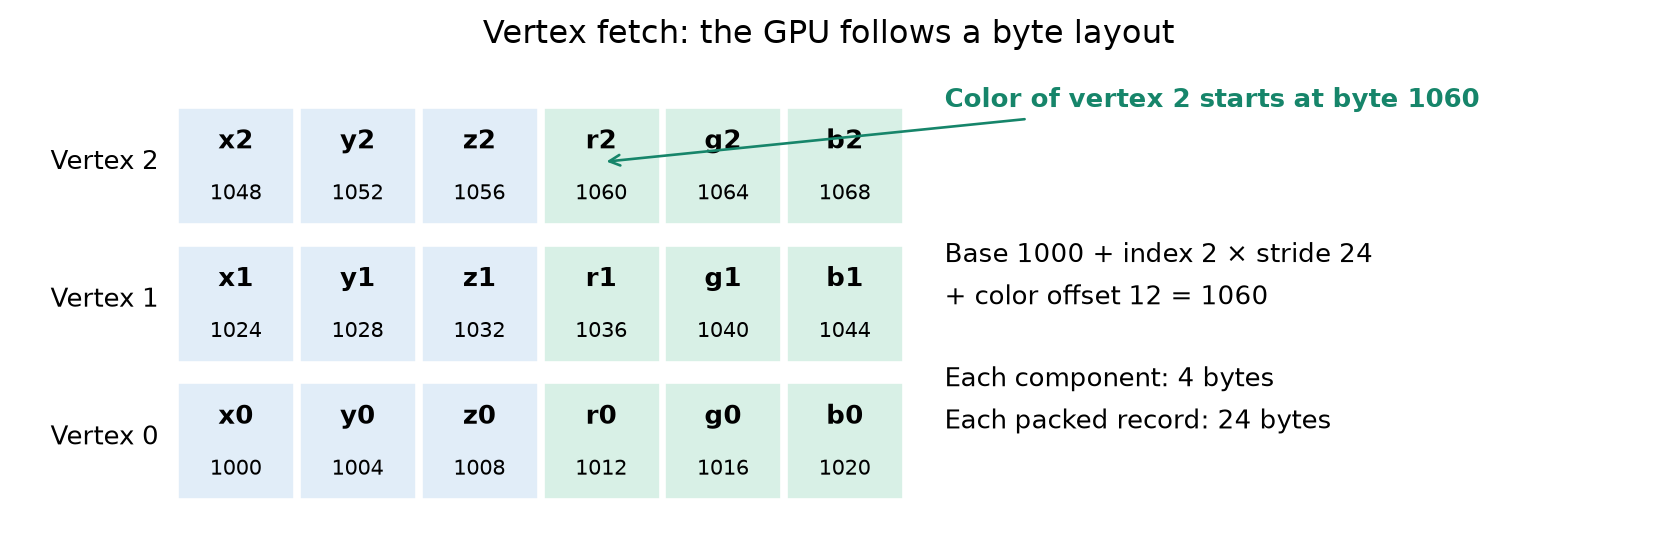
\includegraphics[keepaspectratio,alt={Visual Recall/University Graphics and Vision/vertex-byte-fetch.png}]{Visual Recall/University Graphics and Vision/vertex-byte-fetch.png}}
\caption{Visual Recall/University Graphics and Vision/vertex-byte-fetch.png}
\end{figure}

\emph{This checked example uses packed float32 positions and colors, a 24-byte vertex stride, and a color offset of 12 bytes. It illustrates one memory layout, not every GPU format or binding model.}

\begin{center}\rule{0.5\linewidth}{0.5pt}\end{center}

\hyperref[volume-reading-map]{Reading map} · \hyperref[03-visual-computing-i-ch017]{Previous chapter} · \hyperref[03-visual-computing-i-ch019]{Next chapter}
